\documentclass[tikz,border=12pt]{standalone}

\usepackage{amsmath}
\usepackage{bm}
\usetikzlibrary{calc,arrows.meta}

\begin{document}

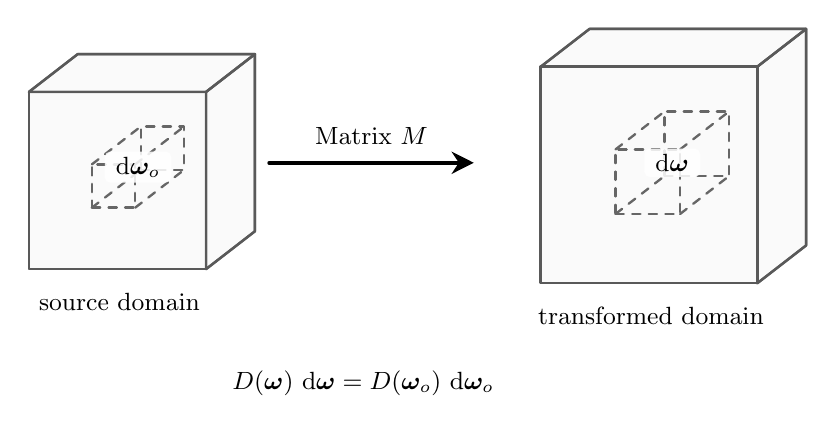
\begin{tikzpicture}[
    line cap=round,
    line join=round,
    >=Stealth,
    font=\small
]

% ============================================================
% Parameters
% ============================================================

\def\dx{0.62}
\def\dy{0.48}

% ============================================================
% Styles
% ============================================================

\tikzset{
    outer face/.style={
        draw=black!55,
        line width=0.85pt,
        fill=gray!18,
        fill opacity=0.20
    },
    outer edge/.style={
        draw=black!65,
        line width=0.9pt
    },
    inner edge/.style={
        draw=black!60,
        dashed,
        line width=0.85pt
    },
    arrowstyle/.style={
        -{Stealth[length=8pt,width=8pt]},
        line width=1.25pt,
        draw=black
    },
    labelbox/.style={
        fill=white,
        fill opacity=0.86,
        text opacity=1,
        rounded corners=2pt,
        inner xsep=4pt,
        inner ysep=2pt,
        align=center
    },
    formula/.style={
        fill=white,
        fill opacity=0.94,
        text opacity=1,
        rounded corners=3pt,
        inner xsep=8pt,
        inner ysep=5pt,
        align=center
    }
}

% ============================================================
% Draw a cube
% #1 origin
% #2 side length
% #3 prefix
% ============================================================

\newcommand{\DrawCube}[3]{%
    \coordinate (#3A) at #1;
    \coordinate (#3B) at ($(#3A)+(#2,0)$);
    \coordinate (#3C) at ($(#3A)+(0,#2)$);
    \coordinate (#3D) at ($(#3A)+(#2,#2)$);

    \coordinate (#3Ap) at ($(#3A)+(\dx,\dy)$);
    \coordinate (#3Bp) at ($(#3B)+(\dx,\dy)$);
    \coordinate (#3Cp) at ($(#3C)+(\dx,\dy)$);
    \coordinate (#3Dp) at ($(#3D)+(\dx,\dy)$);

    % three visible faces
    \filldraw[outer face] (#3A) -- (#3B) -- (#3D) -- (#3C) -- cycle;
    \filldraw[outer face] (#3B) -- (#3Bp) -- (#3Dp) -- (#3D) -- cycle;
    \filldraw[outer face] (#3C) -- (#3D) -- (#3Dp) -- (#3Cp) -- cycle;

    % visible edges
    \draw[outer edge] (#3A) -- (#3B) -- (#3D) -- (#3C) -- cycle;
    \draw[outer edge] (#3B) -- (#3Bp) -- (#3Dp) -- (#3D);
    \draw[outer edge] (#3C) -- (#3Cp) -- (#3Dp);
}

% ============================================================
% Draw dashed inner cube
% #1 origin
% #2 side length
% #3 prefix
% ============================================================

\newcommand{\DrawInnerCube}[3]{%
    \coordinate (#3A) at #1;
    \coordinate (#3B) at ($(#3A)+(#2,0)$);
    \coordinate (#3C) at ($(#3A)+(0,#2)$);
    \coordinate (#3D) at ($(#3A)+(#2,#2)$);

    \coordinate (#3Ap) at ($(#3A)+(\dx,\dy)$);
    \coordinate (#3Bp) at ($(#3B)+(\dx,\dy)$);
    \coordinate (#3Cp) at ($(#3C)+(\dx,\dy)$);
    \coordinate (#3Dp) at ($(#3D)+(\dx,\dy)$);

    % front square
    \draw[inner edge] (#3A) -- (#3B) -- (#3D) -- (#3C) -- cycle;

    % back square
    \draw[inner edge] (#3Ap) -- (#3Bp) -- (#3Dp) -- (#3Cp) -- cycle;

    % connecting edges
    \draw[inner edge] (#3A) -- (#3Ap);
    \draw[inner edge] (#3B) -- (#3Bp);
    \draw[inner edge] (#3C) -- (#3Cp);
    \draw[inner edge] (#3D) -- (#3Dp);
}

% ============================================================
% Left cube
% ============================================================

\begin{scope}[shift={(-4.3,0)}]
    \DrawCube{(0,0)}{2.25}{L}

    \DrawInnerCube{(0.80,0.78)}{0.55}{Li}

    \node[labelbox] at ($(0.80,0.78)+(0.275,0.275)+(0.31,0.24)$)
    {$\mathrm{d}\boldsymbol{\omega}_o$};

    \node at (1.15,-0.42) {source domain};
\end{scope}

% ============================================================
% Right cube
% ============================================================

\begin{scope}[shift={(2.2,-0.18)}]
    \DrawCube{(0,0)}{2.75}{R}

    \DrawInnerCube{(0.95,0.88)}{0.82}{Ri}

    \node[labelbox] at ($(0.95,0.88)+(0.41,0.41)+(0.31,0.24)$)
    {$\mathrm{d}\boldsymbol{\omega}$};

    \node at (1.40,-0.42) {transformed domain};
\end{scope}

% ============================================================
% Arrow
% ============================================================

\draw[arrowstyle]
    (-1.25,1.35) -- (1.35,1.35)
    node[midway, above=4pt, labelbox]
    {Matrix $M$};

% ============================================================
% Formula
% ============================================================

\node[formula] at (0,-1.45)
{
$
D\!\left(\boldsymbol{\omega}\right)\,
\mathrm{d}\boldsymbol{\omega}
=
D\!\left(\boldsymbol{\omega}_o\right)\,
\mathrm{d}\boldsymbol{\omega}_o
$
};

\end{tikzpicture}

\end{document}